
Starting with Rutherford's gold foil experiment, scattering
experiments that measure the deflection of particles in the presence
of some form of matter have been effective in probing the structure of
matter and the forces with which it interacts. Such experiments have
proved to be invaluable testing grounds for the SM. The gauge
structure of the SM has historically been tested by either looking for
evidence of particles introduced in the process of enforcing gauge
symmetry, if those particles had not yet been observed, or if they
had, by measuring the degree to which gauge bosons couple to
fermions and themselves. The coupling strength between fields is
related to a quantity called the cross section which is a measure of
the probability with which a scattering process occurs. For the
scattering of two particles into $n$ particles, the cross section can
be written

\begin{equation}
\hat{\sigma}_{qq\rightarrow{n}} = \int_{\mathscr{V}_n} |M(q_1,q_2;y_1,...,y_n)|^2
d\Phi_n(q_1+q_2;y_1,...,y_n)
\label{chapter:theory:equation:cross_section}
\end{equation}

\noindent
where the $q_i$ ($y_i$) are the momentum 4-vectors of the incoming
(outgoing) particles. The differential $d\Phi_n(q_1+q_2;y_1,...,y_n)$ is the Lorentz
invariant phase space term that enforces conservation of energy and
momentum, and $M(q_1,q_2;y_1,...,y_n)$ is the matrix element that
captures the dynamics of the Lagrangian. It is calculated with the
perturbative techniques of QFT. Therefore, measuring the cross
section $\hat{\sigma}$ for a given scattering process is an effective
test of the relevant terms in the Lagrangian. 

\begin{figure}[h]
\centering
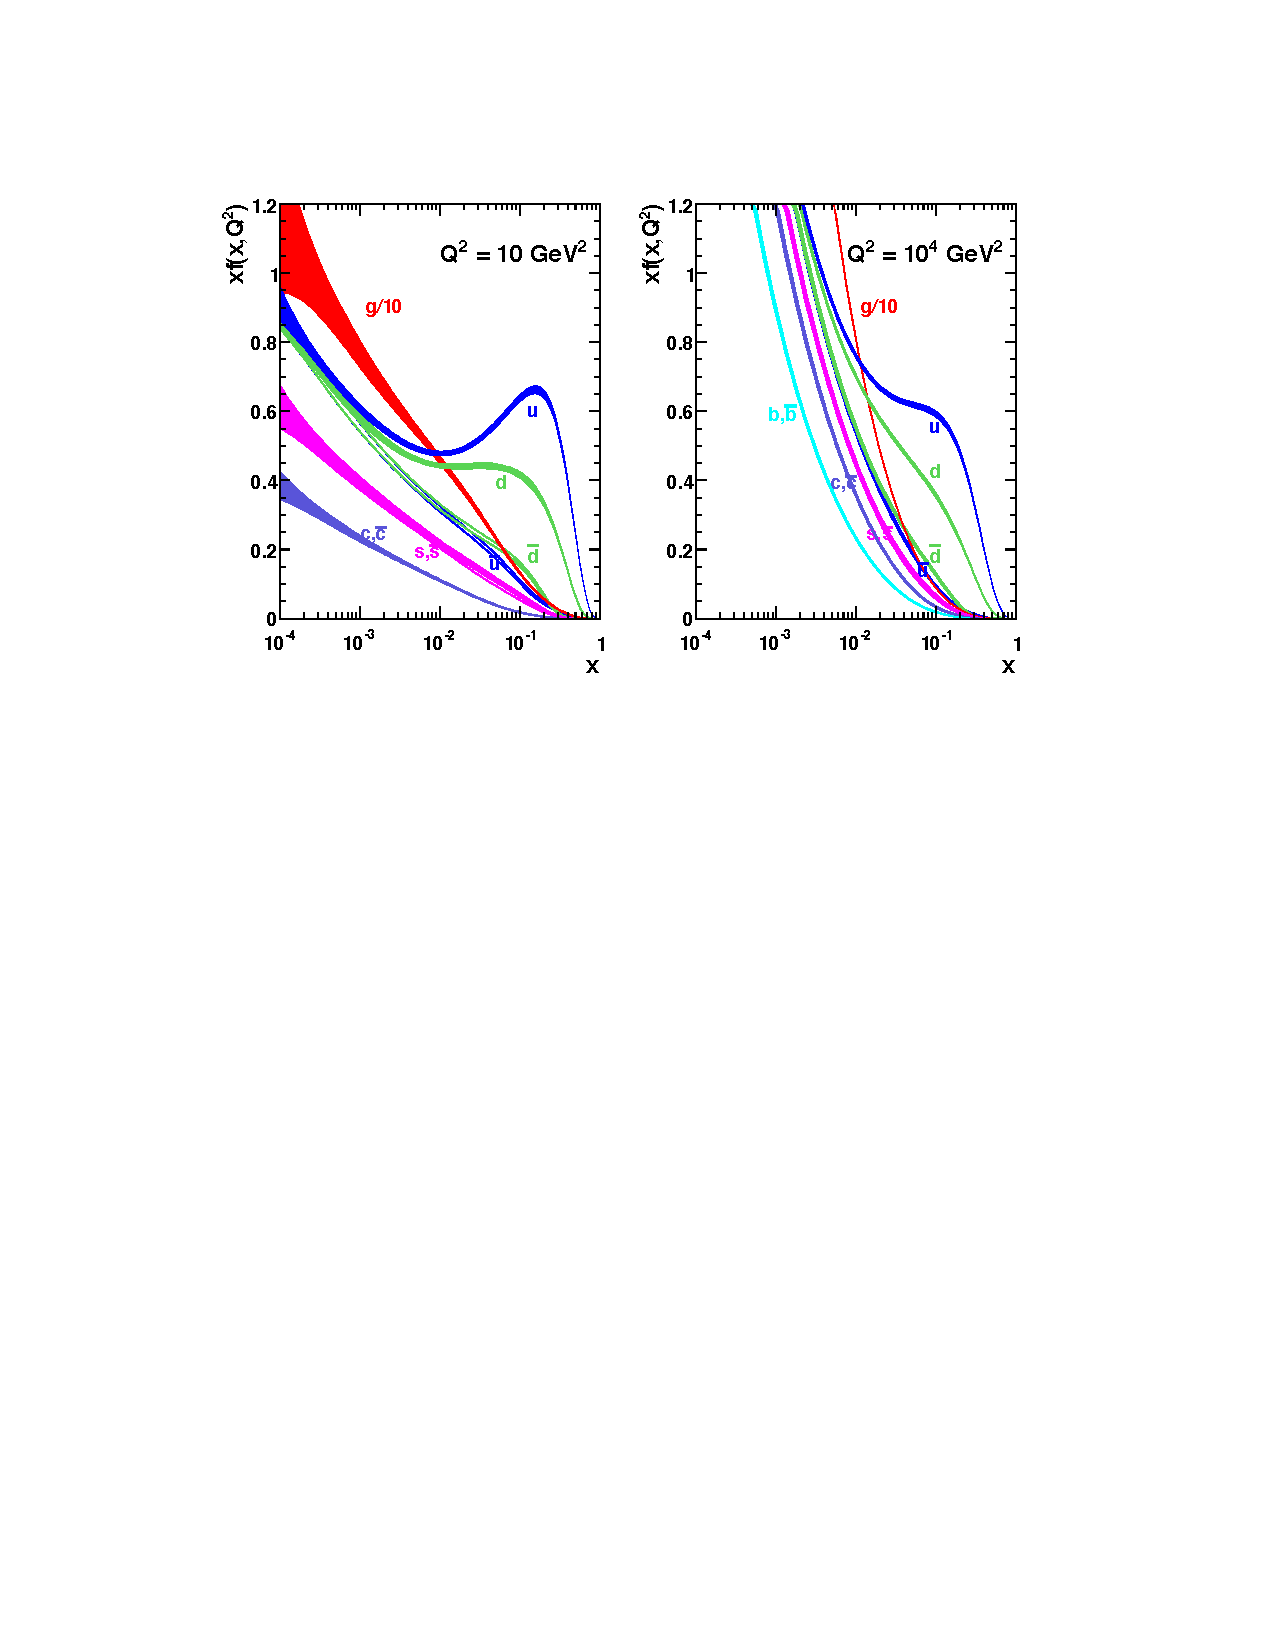
\includegraphics[width=1.0\textwidth]{fig/theory/mstw_pdfs.pdf}
\caption{\cite{bib:Martin:2009iq}}
\label{chap:theory:fig:pdf_set}
\end{figure}

The expression for $\sigma$ defined in
equation~\ref{chapter:theory:equation:cross_section} applies to the
scattering of two elementary particles into $n$ particles. At the LHC,
the two incident particles are protons, which are composite particles
composed of quarks interacting through gluon exchange. Due to the
non-Abelian structure of the gauge group governing these interactions,
as well as the fact that gluons are massless, quarks and gluons can be
described as free particles at sufficiently high energy scales. This
phenomenon, a consequence of the fact that the strong coupling
constant decreases with increasing energy scales, is called
``asymptotic freedom''. It allows the perturbation techniques of QFT
to be used for QCD predictions at energy scales above
$\Lambda_{\textrm{QCD}}$. Below this scale, heuristic non-perturbative
models are used. Particles that are composed of quarks, such as
protons, must have a configuration of two or three quarks that
transforms as an $SU(3)$ color singlet. Protons are composed of three
valence quarks--- two up quarks and a down quark--- as well as a
``sea'' of gluons and quarks of other flavors due to excitations
between the valence quarks. Parton distribution functions (pdfs)
quantify the probability that a given parton within the proton carries
a momentum fraction $x$ of the total proton momentum. These pdfs have
been determined as a function of the energy scale at
which the proton is probed through a global fit of data from deep inelastic scattering (DIS) and
other high energy collider experiments~\cite{bib:Martin:2009iq}. In
figure~\ref{chap:theory:fig:pdf_set}, the results of these fits are
shown as the product of the parton momentum fraction and the pdf,
$xf(x,Q^2)$, which represents the momentum density for a given
parton. At high $x$, the valence quarks carry the majority of the
momentum, and at low $x$ the sea partons begin to contribute momentum,
with the gluon pdf dramatically larger than the others (note that the
gluon distribution is scaled down by a factor of 10). This behavior
turns out to be important in Higgs physics at the LHC
(section~\ref{chapter:theory:section:higgs_physics}).

For proton-proton scattering, the cross section
is computed by weighting the quark-quark scattering cross
sections (e.g. equation~\ref{chapter:theory:equation:cross_section})
by the pdfs and integrating over the momentum fractions:

\begin{equation}
\sigma_{pp\rightarrow{n}} = \int dx_1 dx_2 f_{q_1}(x_1,\mu_F)
  f_{q_2}(x_2,\mu_F) \hat{\sigma}_{qq\rightarrow{n}}.
\label{chapter:theory:equation:cross_section_pp}
\end{equation}

\noindent
Here, $f_{q_1}$ ($f_{q_2}$) is the pdf for a quark of
flavor $q_1$ ($q_2$) and momentum fraction $x_1$ ($x_2$). The cross
section is now expressed in terms of the perturbative cross section
associated with the free partons, with the non-perturbative part
factorized into the pdfs. The scale that separates the two regimes is
called the factorization scale, $\mu_F$. As more terms are included in
the perturbative expansion of $\hat{\sigma}_{qq\rightarrow{n}}$,
divergences arise when, for example, QCD radiation is soft or
collinear. To make the theory predictive again,
$\hat{\sigma}_{qq\rightarrow{n}}$ is renormalized at some scale
$\mu_R$. The resulting cross section calculated at all orders in
perturbation theory is invariant with respect to changes in $\mu_F$
and $\mu_R$. However, due to calculational difficulties, the cross
section is computed at fixed order in perturbation theory,
making it necessary to vary $\mu_F$ and $\mu_R$, and quantify the
change in the predicted cross section. This change is then assigned as
an experimental uncertainty. 

In most scattering experiments, a prediction is obtained from Monte
Carlo (MC) simulation, whereby an event is generated probabilistically
by drawing from the differential cross section distribution defined
by~\ref{chapter:theory:equation:cross_section_pp}. MC generators are
able to generate a hard scattering up to some fixed order, and to augment
fixed order calculations, parton shower (PS) programs are typically
interfaced to the MC generator, allowing diagrams with more vertices
to be modeled. For a quark or gluon in the final state, the PS program
uses the DGLAP equation~\cite{} to model the emission of additional
quarks and gluons down to some cut-off energy scale in a process known
as fragmentation. The resulting partons, which are not confined to color
singlet configurations, are then hadronized using a non-perturbative
model, forming a collection of hadrons that are observable to the
detector. The shower of hadrons associated with a final state quark or
gluon is known as a jet (discussed in more detail in
chapter~\ref{chapter:reconstruction}).

In the electroweak sector of the SM, the gauge structure is tested by
measuring evidence for diagrams that only arise when gauge
invariance is imposed, and by comparing the cross sections of such
processes to the SM predictions. The LHC, with its high
center-of-mass energy, is sensitive to many of these processes, as
shown in figure~\ref{chap:theory:fig:xs_summary_plot}, which
summarizes the cross sections measured by the ATLAS detector for some
important SM processes. The production of a single $W$ or $Z$ boson is
precisely measured to be consistent with the SM prediction. Processes
involving the production of two weak gauge bosons--- $WW$, $WZ$, and
$ZZ$--- are also in agreement with the SM. Such self-consistent
predictions provide strong evidence for the gauge structure of the
SM. 

\begin{figure}
\centering
\includegraphics[width=1.0\textwidth]{fig/theory/ATLAS_c_SMSummary_TotalXsect_rotated.eps}
\caption{}
\label{chap:theory:fig:xs_summary_plot}
\end{figure} 

